%1) Spécification de l’environnement 
%        2) Specification du logiciel : Generation Controlée
%                2.1 Fonctionnalité
%                2.2 Decompo fonctionnelle
%        3) Conception fonctionnelle
%        4) Definition de la réalisation 
%        5) Réalisation 
%        6) Tests
\chapter*{Introduction}
	Ceci est une intro. Hello world!

\chapter{Générateur de tâches}
	\label{chap:1}
	
	\section{Spécification de l’environnement}
	
	Cette application offre la possibilité de créer un fichier contenant un jeu de tâches (périodiques et apériodiques non critiques).
	Dans un premier temps, le programme permet de générer manuellement ce jeu de tâche en offrant une interface minimaliste.
	Dans un deuxième temps, il est possible de générer automatiquement ce fichier en fournissant des contraintes à respecter pour les tâches périodiques et apériodiques.
	
	
	Lorsque le programme est lancé, l’utilisateur doit choisir le mode de génération. Il rentre les données nécessaires au bon déroulement du mode. Le programme crée un fichier qui contient le résultat de la génération de tâches.


	\section{Spécification du logiciel}

		\subsection{Explication du choix du langage}
	
			\label{sec:langage}
			Nous avons opté pour le langage C++ pour réaliser ce projet car celui-ci possède un certain nombre d'avantages. Il s'agit d'un langage orienté objet très utilisé dans le monde et de nombreux outils libres sont disponibles pour l'utiliser (comme GCC pour la compilation par exemple). De plus, la documentation correspondante est très facilement accessible dans la littérature ou sur le web.
		
			Bien que le travail qui nous a été demandé ne requiert pas la maîtrise d'une programmation bas niveau, le langage C++ nous apparait en cohérence avec le thème abordé par le projet (les systèmes temps réel embarqués).

		\subsection{Fonctionnalités}
			\begin{figure}
				\centering
				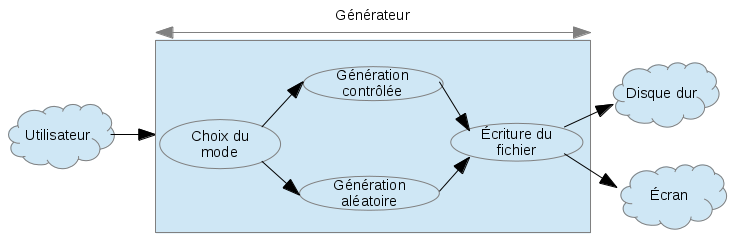
\includegraphics[scale=0.9]{img/schema_gen.png}
				\caption{Fonctionnement et modules du générateur.}
			\end{figure}
			\FloatBarrier
		    
			\subsubsection{Choix du mode}
				Dans ce premier module, on choisit le mode d’utilisation du logiciel en fonction de ce que souhaite l’utilisateur. Pour cela, il peut soit renseigner sous forme d’arguments les différentes données, soit en sélectionnant dans le menu ses préférences. \\

				Parmi les choix qui lui sont offerts, on retrouve les cas présentés dans le sujet du projet (génération aléatoire ou contrôlée et tâches périodiques ou non) mais aussi la possibilité de renseigner un fichier contenant déjà toutes les informations sur les tâches. Dans le premier cas, l’utilisateur devra renseigner ensuite le nombre de tâches concernées tandis que dans l’autre cas, le fichier ne sera pas interprété et ce programme s’arrêtera.


			\subsubsection{Génération aléatoire de tâches}
				Le premier type de génération permet de générer automatiquement des tâches. L'utilisateur devra renseigner le nombre de tâches périodiques et apériodiques à générer ainsi que le pourcentage d'utilisation du CPU. Ceci permet de générer des fichiers de test aléatoire qui seront visualisable par la suite.\\
				Lors de la génération, le système calcule les différentes valeurs caractéristiques des tâches périodiques (Ci, Pi, Di) et des tâches apériodiques (ri, Ci) en accord avec le pourcentage d'utilisation du CPU. 

			\subsubsection{Génération contrôlée de tâches}
				Le deuxième type de génération fait appel à l'utilisateur pour renseigner chacune des valeurs de chaque tâche. De cette manière, l'utilisateur va pouvoir tester plus facilement des cas spécifiques et donc observer de manière plus précise le fonctionnement de l'ordonnanceur par la suite. \\
				Lors de la génération, pour toutes les tâches périodiques il devra renseigner les Ci, Pi et Di, c'est-à-dire respectivement les durées d'exécution maximales, les périodes d'activation et le délai critique). Dans le cas où il y a aussi des tâches apériodiques, il devra renseigner aussi ri (la date de réveil) et Ci.

			\subsubsection{Écriture dans un fichier}
				Ce module a pour fonction d’écrire dans un fichier les données contenues dans un flux (= stream)  et calculées à partir des deux modules précédents de génération. L’intérêt de séparer ces fonctions est double : il est plus pratique de factoriser le code à travers une seule fonction d’écriture appelée par les différentes générations et cela facilite la maintenance.


		\subsection{Décomposition fonctionnelle}
			Une classe par type de génération 


	\section{Conception fonctionnelle}

		\subsection{Choix du mode}
			\paragraph{Pré-condition :} Le programme vient d’être lancé.
			\paragraph{Post-condition :} Un choix valide a été effectué.
			\paragraph{Objectif :} Permettre de choisir entre la génération aléatoire et la génération controlée.
			\paragraph{Algo :}
			\begin{verbatim} 
	Entrée : Int choix
	Sortie :  -

Si (choix == 1 ) Alors
   Lancer la génération controlée
Sinon
   Si (choix == 2) Alors
	  Lancer la génération aléatoire 
   Sinon
	  Si (choix == 3) Alors
	     Quitter le programme
	  Sinon
	     Afficher erreur de choix 
	  FinSi
   FinSi
FinSi
		\end{verbatim} 

	\newpage
	\subsection{Génération Aléatoire}
		\paragraph{Pré-condition :} La génération aléatoire a été choisie.
		\paragraph{Post-condition :} Toutes les valeurs caractéristiques des tâches ont été générées en accord avec le paramétrage de l’utilisateur.


		\paragraph{Objectif :} Générer aléatoirement les caractéristiques (Ci,Pi,Di) d’un nombre de tâches (determiné par l’utilisateur) en accord avec un facteur d’utilisation du processeur (déterminé lui aussi par l’utilisateur).
		Ex : pour trois taches et facteur = 75\% \\ 


		    Tirage aléatoire de trois nombres ( 35, 25, 15) dont la somme vaut 75. \\
		    Ces nombres représentent le rapport Ci/Pi dans la formule  \\
		    Il faut ensuite donner une valeur à Ci et Pi. Pour cela, on trouve le pgcd du nombre et de 100. Pour C1/P1 = 35, on obtient 5.  on affecte à C1 $\leftarrow$ 35/5 et à P1 $\leftarrow$ 100/5 , on obtient donc C1 = 7 et P1 = 20. On considère, dans ce programme que Pi = Di. \\
		    
		    On obtient donc dans cette exemple :  \\
		    T1(7,20,20) \\
		    T2(1,4,4) \\
		    T3(3,20,20) \\

		    Toutes les données sont stockées dans 3 tableaux (un pour les Ci, un pour Pi, un pour Di). 

		\paragraph{Algo :}
			\begin{verbatim}
Entrée: Int nbTaches, Int factUtProcesseur
Sortie : 3 Tableaux d’Int (pour les valeurs de Ci, Pi, Di). 
indice du tableau = numéro de la tâche - 1..

TabCi[ nbTaches ], TabPi[ nbTaches ], TabDi[ nbTaches ]
nbTachesRestantes = nbTaches - 1
nbMax = factUtProcessus 

/*
On calcule la valeur maximale que peut prendre le nombre tiré aléatoirement :
maximum = Up - somme des Ci/Pi précédents - nombre de taches restantes
Ensuite, on tire au hasard une valeur allantDe 1 a cette valeur maximale.
Exemple : maxT1 = 75 - 0 - 2
	    randT1 = 32 (valeur calculée avec le pseudo-hasard)
	    maxT2 = 75 - 32 - 1
	    randT2 = 18
	    maxT3 = 75 - (32 + 18) - 0
	    randT3 = 25
Pour résumer, on obtient ici les Ci/Pi : 32, 18 et 25
*/


Pour i allantDe 0 a (nbTaches - 1)
   nbMaxLimite = nbMax - nbTachesRestantes
   // le nombre aléatoire correspond a (Ci/Pi)
   nbAleatoire = nombre Aleatoire entre 1 et ce nombre maximum


   // On calcule et stocke la valeur des Ci, Pi et Di dans 3 tableaux distincts
   tabCi[i] = nb\_genere / pgcd(nb\_genere,100)
   tabPi[i] =100 / pgcd(nb\_genere,100)
   tabCi[i] = 100 / pgcd(nb\_genere,100)
	        
   /* On abaisse ensuite la limite pour le prochain tirage aléatoire afin de ne jamais dépasser la valeur de Up. */
   limite\_maj = limite\_maj - nb\_genere
Fin du pour

// Pour la dernière tâche, on ne génère pas de valeur. On prend ce qu’il reste.
nb\_genere = limite\_maj
tabCi[ nbTaches - 1 ] = nb\_genere / pgcd(nb\_genere,100)
tabPi[ nbTaches - 1 ] =100 / pgcd(nb\_genere,100)
tabCi[ nbTaches - 1 ] = 100 / pgcd(nb\_genere,100)
			\end{verbatim}

	\subsection{Generation Controlée}  
		\paragraph{Pré-condition :} La génération controlée a été choisie.
		\paragraph{Post-condition :} Toutes les valeurs caractéristiques des tâches ont été générées en accord avec le paramétrage de l’utilisateur.
		\paragraph{Objectif :} Permettre à l’utilisateur de générer des tâches périodiques ou apériodiques en renseignant les différentes caractéristiques de chacune des tâches (Ci, Pi, Di) ou, respectivement, (ri, Ci).
		\paragraph{Algo :} 
			\begin{verbatim}
Entrée : Int nbTaches
Sortie :  3 Tableaux d’Int (pour les valeurs de Ci, Pi, Di). 
indice du tableau = numéro de la tâche - 1 .

//génération des tâches périodiques
lire(nbTachesPeriodiques)

TabCiP[ nbTachesPeriodiques ], TabPiP[ nbTachesPeriodiques ], TabDiP[ nbTachesPeriodiques ]
		
Pour i allantDe 0 a (nbTachesPeriodiques - 1)
	// on demande a l’utilisateur de renseigner les différentes valeurs ...
	lire(CiP)
	lire(PiP)
	lire(DiP)        
	// … et on les insére dans les tableaux respectifs
	tabCiP[ i ] = CiP
	tabPiP[ i ] = PiP
	tabDiP[ i ] = DiP
fin pour

//génération des tâches Aperiodiques
lire(nbTachesAperiodiques)

TabriA[ nbTachesAperiodiques ], TabCiA[ nbTachesAperiodiques ]
		
Pour i allantDe 0 a (nbTachesAperiodiques - 1)
	// on demande a l’utilisateur de renseigner les différentes valeurs ...
	lire(riA)
	lire(CiA)        
	// … et on les insére dans les tableaux respectifs
	tabriA[ i ] = riA
	tabCiA[ i ] = CiA
fin pour

			\end{verbatim}

	\subsection{Ecriture du résultat obtenu}
		\paragraph{Pré-condition :} La génération (qu'elle soit contrôlée ou non) envoie un outputstream contenant les chaînes de caractère à écrire dans un fichier.
		\paragraph{Post-condition :} L'écriture s'est bien déroulée : le fichier contient bien la chaîne.
		\paragraph{Objectif :} Enregistrer les données générées par le module précédent de manière pérenne dans un fichier.
		\paragraph{Algo :}
		\begin{verbatim}
création du fichier

	outputstream ops = ""
Pour i allantDe 0 a (nbTachesPeriodiques - 1)		
	ops << "T" << (i+1) << ": " << tabCiP[i] << "," << tabPiP[i] << "," << tabDiP[i] << endl
Finpour

Pour i allantDe 0 a (nbTachesAperiodiques - 1)
	ops << R" << (i+1) << ": " << tabriA[i] << "," << tabCiA[i] << endl
Finpour

écriture dans le fichier de ops
  
		\end{verbatim}

\section{Réalisation}
	\subsection{Choix d'implémentation des structures}
	
	\subsection{Problèmes rencontrés}

\section{Tests}



\chapter{Simulateur d'ordonnanceur}
	\section{Spécification de l’environnement}
		Cette application s'incrit à la suite du générateur de tâches. Elle offre, après récupération des informations du fichier issus du générateur, la possibilité de vérifier l'ordonnançabilité d'un jeu de tâches fournie. Ceci nous permet de savoir si les contraintes temporelles sont respectées. 

	La deuxième fonctionnalité de ce programme est d'offrir un environnement de simulation selon plusieurs politiques d'ordonnancements :
	\begin{itemize}
		\item pour les tâches périodiques : \textbf{RM} et \textbf{EDF}
		\item pour les tâches apériodiques non critiques :  \textbf{BG} et \textbf{TBS}
	\end{itemize}
	Cet environnement, après simulation, fourni à l'utilisateur des résultats de performances relatifs à l'ordonnancement : 
	\begin{itemize}
		\item le nombre de commutations de contexte,
		\item le nombre de préemptions
		\item les temps de réponse des tâches apériodiques.
	\end{itemize}
	
	A la suite de la simulation, le programme doit fournir un fichier de trace de la séquence d'ordonnancement. Ce fichier est au format "ktr" et est exploitable par l'outil Kiwi. 
	Kiwi est un outil graphique développé à l'Université polytechnique de Valence en Espagne. Il permet, à partir d'un fichier texte normé, d'afficher un graphe d'ordonnancement. Nous détaillerons par la suite le contenu du fichier de trace mais il est important pour la suite de savoir que le fichier doit être remplit de manière chronologique.
		
	Le programme final devra pouvoir être exécutable en ligne de commande.\\
		
	En entrée : le nom du fichier contenant le jeu de tâches périodiques et apériodiques pour lesquelles on veut simuler l'ordonnancement.\\
		
	En sortie : un ou plusieurs fichiers .ktr utilisable avec l'outil Kiwi et contenant la séquence d'ordonnancement. Le programme affichera également quelques résultats via la sortie standard.\\
		
		Afin de faciliter la prise en main du programme, on proposera un menu succint présentant les différentes fonctionnalités qui s'offrent à l'utilisateur.
	
	\section{Spécification du logiciel}
		Pour les mêmes raisons que celles décrites dans le Chapitre \ref{sec:langage}, le langage utilisé est le C++.

		\subsection{Fonctionnalité}
			\begin{figure}
				\centering
				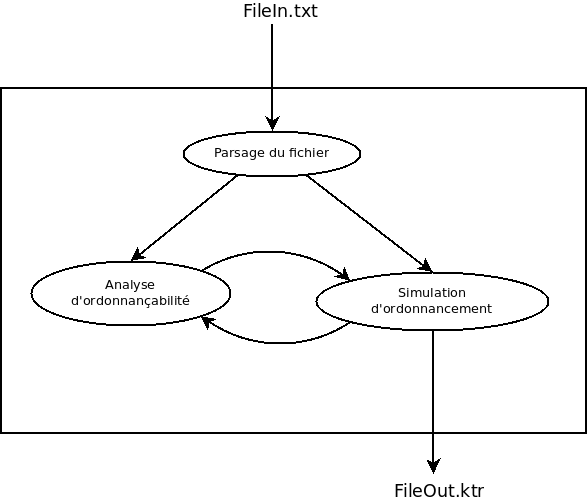
\includegraphics[scale=0.55]{ordo_fct_diag.png}
				\caption{Diagramme des fonctionnalités}
			\end{figure}
			\FloatBarrier
			
			\subsubsection{Parsage du fichier d'entrée}
				Vérification de la syntaxe avec expression régulière + enregistrement des tâches et de leurs paramètres dans un modèle.
			
			\subsubsection{Analyse d'ordonnançabilité}
				{\Huge TODO ajouter les tests pour les taches périodiques où Di < Pi}
				On fait tous les calculs en même temps :
				\begin{itemize}
					\item Condition nécessaire pour l'ordonnançabilité du jeu de tâches avec RM ;
					\item Condition suffisante avec RM ;
					\item Condition suffisante et nécessaire avec EDF.
				\end{itemize}
			
			\subsubsection{Simulation d'ordonnancement}
				
			
			\subsubsection{Ecriture du fichier de trace}
				Pendant la simulation de l'ordonnancement, l'application génére les différentes lignes qui composent le fichier de trace exploitable par Kiwi. Ce fichier se décompose en 2 parties :
					\begin{itemize}
						\item Une entête contenant la déclaration des tâches et la durée d'ordonnancement (hyperpériode)
						\item Les évènements concernants les tâches dans l'ordre chronologique.
					\end{itemize}
		\subsection{Decomposition fonctionnelle}

	\section{Conception fonctionnelle}
		
		\subsection{choix de représentation}
			Nous avons choisi de représenter une temps par l'indice -1
						
		\subsection{Analyse du fichier d'entrée}
				\paragraph{Post-condition :} 
				\paragraph{Objectif :} 
				\paragraph{Algo :} 
					\begin{verbatim}
ALGO TODO
					\end{verbatim}
		
		
		\subsection{Analyse d'ordonnançabilité}
			
			\subsubsection{Condition nécessaire RM}
				\paragraph{Pré-condition :} $n$ représente le nombre de tâches périodiques.
				\paragraph{Post-condition :} Soit c'est non-ordonnançable, soit on ne peut rien conclure.
				\paragraph{Objectif :} Vérifier les conditions d'ordonnançabilité nécessaires pour l'algorithme RM.
				\paragraph{Algo :} 
					\begin{lstlisting}
U = 0
					
Pour i de 0 a n faire
	U = U + Ci/Pi
Finpour		

Si U <= 1.0 alors
	afficher("On ne peut rien conclure")
Sinon
	afficher("Non-ordonnancable")
Finsi
					\end{lstlisting}
			
			\subsubsection{Condition suffisante RM}
				\paragraph{Pré-condition :} $n$ représente le nombre de tâches périodiques.
				\paragraph{Post-condition :} Soit c'est ordonnançable, soit on ne peut rien conclure.
				\paragraph{Objectif :} Vérifier les conditions d'ordonnançabilité suffisantes pour l'algorithme RM.
				\paragraph{Algo :} 
					\begin{lstlisting}[mathescape]
U = 0
UBoundRM = $n * (2^{(1.0 / n)} - 1)$
					
Pour i de 0 a n faire
	U = U + Ci/Pi
Finpour

Si U <= UBoundRM alors
	afficher("Ordonnancable")
Sinon
	afficher("On ne peut rien conclure")
Finsi
					\end{lstlisting}
			
			\subsubsection{Condition nécessaire et suffisante EDF}
				\paragraph{Pré-condition :} $n$ représente le nombre de tâches périodiques et il n'y a pas de tâches apériodiques.
				\paragraph{Post-condition :} On obtient une réponse binaire : le système est ordonnançable ou non.
				\paragraph{Objectif :} Vérifier les conditions d'ordonnançabilité nécessaires et suffisantes pour l'algorithme EDF.
				\paragraph{Algo :} 
					\begin{lstlisting}[mathescape]
egaliteDiPi = vrai					
superioritePiDi = vrai
U = 0		
			
pour i de 0 a n faire
    // Verifie si tous les Pi sont bien egaux aux Di
	egaliteDiPi &= (Pi == Di) 
	// idem pour Pi > Di
	superioritePiDi &= (Pi > Di) 
Finpour

Si egaliteDiPi alors
	afficher "Test de condition necessaire et suffisante pour EDF : "

    Pour i de 0 a n faire
	    U = U + Ci/Pi
    Finpour
	
	Si (U <= 1.0) alors
		afficher "ordonnancable"
	Sinon
		afficher "non-ordonnancable"
	Finsi
	
Sinon Si superioritePiDi alors
	afficher "Test de condition suffisante pour EDF : "
    
    Pour i de 0 a n faire
	    U = U + Ci/Di
    Finpour
	
	Si (U <= 1.0) alors
		afficher "ordonnancable"
	Sinon
		afficher "on ne peut rien conclure"
	Finsi
Sinon
    afficher "Erreur : au moins un Pi < Di"
Finsi
					\end{lstlisting}
					
			\subsubsection{Condition nécessaire et suffisante EDF-TBS}
				\paragraph{Pré-condition :} $n$ représente le nombre de tâches périodiques et Us est .
				\paragraph{Post-condition :} On obtient une réponse binaire : le système est ordonnançable ou non.
				\paragraph{Objectif :} Vérifier les conditions d'ordonnançabilité nécessaires et suffisantes pour l'algorithme EDF.
					\begin{lstlisting}
U = 0

Pour i de 0 a n faire
    U = U + Ci/Pi
Finpour
					
afficher "Test de condition necessaire et suffisante pour EDF-TBS : "
Si (Up + Us <= 1.0) alors
	afficher "ordonnancable"
Sinon
	afficher "non-ordonnancable"
Finsi
					\end{lstlisting}
	
		\subsection{Simulation d'ordonnancement}
			Le simulateur d'ordonnancement est découpé en deux algorithmes principaux :
			\begin{itemize}
				\item RM ;
				\item EDF.
			\end{itemize}
			
			Nous avons en premier lieu commencé par développer ces deux algorithmes sans tenir compte des tâches apériodiques dans le but ensuite de les "patcher" avec nos algorithmes d'ordonnancement des tâches apériodiques (BG et TBS).
			
			
			\subsubsection{poll\_needed}
				\paragraph{Pré-condition : un algo d'ordonnancement a été lancé} 
				\paragraph{Post-condition :retourne un booléan qui informe du besoin du besoin d'élire un nouvelle tâche à exécuter} 
				\paragraph{Objectif : Savoir si on doit élire une nouvelle tâche ou non} 
				\paragraph{Algo :} 
					\begin{lstlisting}
					
	bool need_to_poll = false;
	//Ordonnanceur appele que si reveil ou terminaison de tache
		//verification du reveil d'une tache
			//Taches Periodiques
			
			Pour tachePeriodique dans context
				Si time = (date Reveil de tachePeriodique)
					ajout de tachePeriodique dans tabPeriodiquesPretes
					need_to_poll = true
				Finsi
			Finpour
			
			//Taches Aperiodiques
			Si (un serveur de taches a ete specifie) 
				Pour tacheAperiodique dans context
					Si time = (date Reveil de tacheAperiodique)
						ajout de tacheAperiodique dans tabAperiodiquePretes
						need_to_poll = true
						Si (le serveur de tache aperiodique choisi est TBS)
							calcul de dk pour tacheAperiodique
							stockage dans context
						Finsi
					Finsi
				Finpour
			Finsi
			
		//verification de la terminaison de la tache courante executee
		
		Si (la tache courante executee n'est PAS un temps creux)
			Si (la capacite restante de tache courante executee = 0)
				need_to_poll = true
				//Suppression de la tache d'un des tableaux de taches pretes
				Si (la tache courante executee est une tache Aperiodique)
					suppression de la tache de tabAperiodiquesPretes
				Sinon
					suppression de la tache de tabPeriodiquesPretes
				Finsi
		
			Finsi
		Finsi
		
		retourne need_to_poll
				
					\end{lstlisting}
				
			\subsubsection{init\_context}
				\paragraph{Pré-condition :} 
				\paragraph{Post-condition :} 
				\paragraph{Objectif :} 
				\paragraph{Algo :} 
					\begin{lstlisting}

//Initialisation du context : 
 	- creation d'un tableau contenant toutes les taches (taches periodiques puis taches aperiodiques)
 	- le tableau context est un tableau de 3 case de large et nbTaches de long
 	- pour les taches periodiques :
 		. indice -> Capacite restant | prochaine date de reveil | prochaine date echeance
 	- pour les taches aperiodiques : 
 		. indice -> Capacite restante | date de reveil | date echeance ( si TBS sinon 0)
 		 
 context[ nbTaches ] [ 3 ]
 
 Pour i allantDe 0 a nbTachePeriodiques
 	context[i][0] = Ci de tachePeriodique_i
 	context[i][1] = Pi de tachePeriodique_i
 	context[i][2] = Di de tachePeriodique_i
 Finpour
 
 Si (il y a un serveur de precise)
 	Pour i allantDe nbTachesPeriodiques a nbTaches
 		context[i][0] = Ci de tacheAperiodique_i
 		context[i][1] = ri de tacheAperiodique_i
 		context[i][2] = 0 
 	Finpour
 Finsi
					\end{lstlisting}			
					
			\subsubsection{MAJ\_context}
				\paragraph{Pré-condition :} 
				\paragraph{Post-condition :} 
				\paragraph{Objectif :} 
				\paragraph{Algo :} 
					\begin{lstlisting}
					
Pour tachePeriodique dans context
	//verification du depassement d'echeance
	Si (time = (date echeance tachePeriodique) )
		Si ( (capacite restante de tachePeriodique) > 0 )
			Message("Depassement d'echeance pour la tache : T" + tachePeriodique)
			quitter
		Finsi
	Finsi
	
	Si (time = (date reveil de tachPeriodique) )
		capacite restante tachePeriodique = Ci de tachePeriodique
		date de reveil tachePeriodique = date de reveil tachePeriodique + Pi de tachePeriodique
		date echeance tachePeriodique = date echeance tachePeriodique + Di de tachePeriodique
	Finsi
Finpour

//Verification de depassement d'echeance pour les taches aperiodiques
//Si serveur de taches aperiodiques est TBS
	Si (serveur = TBS)
		Pour tacheAperiodique dans context
			Si (time = (deadline de tacheAperiodique) )
				Si ( (capacite restante tacheAperiodique) > 0 )
					Message("Depassement d'echeance pour la tache : R" + tacheAperiodique)
					quitter
				Finsi
			Finsi
		Finpour
	Finsi
Finsi
		
					\end{lstlisting}
			\subsubsection{Rate Monotonic + Serveur}
				\paragraph{Pré-condition :} 
				\paragraph{Post-condition :} 
				\paragraph{Objectif :} 
				\paragraph{Algo :} 
					\begin{lstlisting}
Entree : 
Sortie :  

//Initialisation du context : 
	- Creation d'un tableau de taches periodiques par ordre de prio : tabPrioPeriodique
	- Creation d'un tableau de taches aperiodiques par ordre de prio : tabPrioAperiodique
	- Creation d'un tableau qui contient la capacite restante de chaque tache : tabTpsRestant
init_context()

int t := 0
int task_executed := -1
bool tache_elue = false;

Tantque (t < getHyperPeriode())
	
    Booleen need_to_poll = poll_needed()
	
    Si(need_to_poll)
        tache_elue = false
        Pour taches dans tabPrioPeriodique
        	Si (tabTpsRestant[tache] >0 && tache_elue == false)
        		task_executed = tache;
        		tache_elue = true;
        	Finsi 
        Finpour
        // si Aucune tache n'a ete choisie -> temps creux
        Si tache_elue == false
        	//temps_creux
        Finsi
    finsi
	
	tabTpsRestant[task_executed]--;
    maj_context()
    t++
	
Fintantque
					\end{lstlisting}
					
					
			\subsubsection{Earliest Deadline First + Serveur}
			
				\paragraph{Pré-condition :} 
				\paragraph{Post-condition :} 
				\paragraph{Objectif :} 
				\paragraph{Algo :} 
					\begin{lstlisting}
Entree : 
Sortie :  


init_context()
int t := 0
int task_executed := -1

Tantque (t < getHyperPeriode())
	
	Booleen need_to_poll = poll_needed()
	
	Si(need_to_poll)
		Si (aucune tache periodique prete) 
			Si (aucune tache aperiodique prete)
				temps_creux
			Sinon
				task_executed = Selection de la tache Aperiodique prete dont le ri est le plus petit
			Finsi
		Sinon
			deadlineProche = hyperperiode
			task_executed = temps_creux
			
			//election de la tache Periodique prete la plus prioritaire
			
			Pour tachePeriodiquePrete dans tabPeriodiquesPretes
				Si ( deadlineProche > (prochaine date echeance tachePeriodiquePrete) )
					deadlineProche = prochaine date echeance tachePeridiodiquePrete
					task_executed = tachePeriodiquePrete
				Sinon
					Si ( deadlineProche = (prochaine date echeance tachePeriodiquePrete) )
						//Conflit --> on compare les dates de reveil
						Si ( ri_task_executed > ri_tacheAperiodiquePrete)
							task_executed = tachePeriodiquePrete
						Sinon
							Si (ri_task_executed = ri_tacheAperiodiquePrete)
								// Conflit --> on compare les numeros de tache
								Si (num_task_executed > num_tachePeriodiquePrete)
									task_executed = tachePeriodiquePrete
								Finsi
							Finsi
						Finsi
					Finsi
				Finsi
			Finpour
			
			//election de la tache Aperiodique prete la plus prioritaire
			Si (serveur == TBS)
				Pour tacheAperiodiquePrete dans tabAperiodiquesPretes
					Si ( (dk de tacheAperiodiquePrete) < deadlineProche )
						//La tache Aperiodique est plus prioritaire
						task_executed = tacheAperiodiquePrete
					Sinon
						Si ( (dk de tacheAperiodiquePrete) = deadlineProche )
							Si ( (ri de tacheAperiodiquePrete) < (ri de task_executed) )
								task_executed = tacheAperiodiquePrete
							Finsi
						Finsi
					Finsi
				Finpour
			Finsi
		Finsi
	Finsi
	
	Capacite_restante de task_executed--
	t++
	
	MAJ_context()
	
	
fin tant que
					\end{lstlisting}
				
	\section{Réalisation}
		\subsection{Choix d'implémentation des structures}
	
		\subsection{Problèmes rencontrés}


	\section{Tests}
	
\chapter*{Conclusion}

